\documentclass[tikz,border=2pt]{standalone}
\usepackage{amsmath,amssymb}
\usepackage{tikz}
\usetikzlibrary{arrows.meta}

\begin{document}
% The augmenting path (Ford-Fulkerson) algorithm on the example: start from zero flow and
% augment along three paths until no source-sink path with positive residual capacity exists.
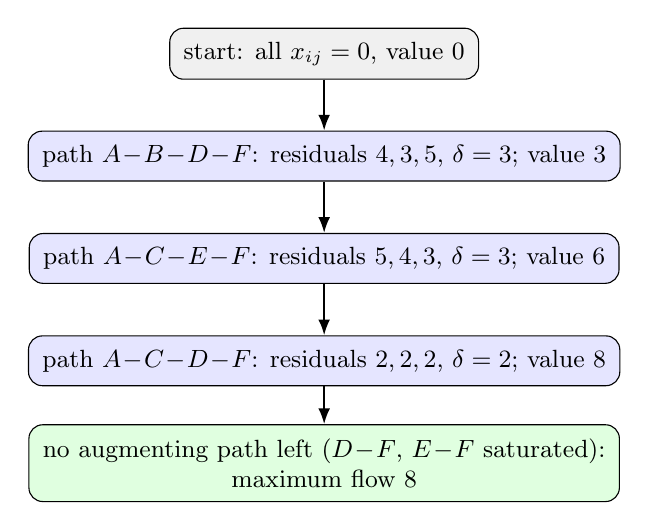
\begin{tikzpicture}[every node/.style={font=\small}, >={Latex[length=2mm]}, st/.style={draw, rounded corners=5pt, inner sep=5pt, align=center}]
	\node[st, fill=gray!12] (s0) at (0,0) {start: all $x_{ij}=0$, value $0$};
	\node[st, fill=blue!10] (s1) at (0,-1.3) {path $A\!-\!B\!-\!D\!-\!F$: residuals $4,3,5$, $\delta=3$; value $3$};
	\node[st, fill=blue!10] (s2) at (0,-2.6) {path $A\!-\!C\!-\!E\!-\!F$: residuals $5,4,3$, $\delta=3$; value $6$};
	\node[st, fill=blue!10] (s3) at (0,-3.9) {path $A\!-\!C\!-\!D\!-\!F$: residuals $2,2,2$, $\delta=2$; value $8$};
	\node[st, fill=green!12] (s4) at (0,-5.2) {no augmenting path left ($D\!-\!F$, $E\!-\!F$ saturated):\\ maximum flow $8$};
	\foreach \a/\b in {s0/s1, s1/s2, s2/s3, s3/s4} {\draw[->, thick] (\a) -- (\b);}
	\end{tikzpicture}
\end{document}
